\citelink{basal}{Basal ganglia is a part of the human brain which is a group of subcortical nuclei responsible primarily for motor control, as well as other roles such as motor learning, executive functions and behaviors, and emotions.} \citelink{hunting}{Huntington’s disease is a disorder that causes the progressive degeneration of the basal nuclei.}\par

Hospital de Bellvitge provided an excellent dataset of anatomocal \ac{MRI} and \ac{DTI} records of 32 control and 38 Huntington patient records of T1 and T1/T2 \ac{MRI} images with isotropic voxels of 1 millimeter resolution and \ac{DTI} \ac{FA}, \ac{MD} and \ac{RD} images with isotropic voxels of 2 millimeter resolution. Furthermore this dataset also contains the mask for the basal ganglia, which will also be referenced as the \ac{ROI}. Masks for the 7 main cortical regions of the brain, which will also be referenced as the target regions: Limbic, Executive, Rostral-Motor, Caudal-Motor, Parietal, Occipital and Temporal are also included in the dataset. Tractography was performed on the \ac{DTI} images to figure out which parts of the \ac{ROI} are connected to which cortical target, in a similar manner to how it was done in this \citelink{conn}{paper}; where the relative connectivity maps are representing the ratio of the number of streamlines to each cortical target. Furthermore, the raw streamline images are also available, where there are a maximum of 5000 streamlines starting from each voxel in the \ac{ROI}. The subcortical segmentation of the Basal Ganglia is also available, for the Caudate, Putamen and Accumbens on the control records. And lastly \ac{FNIRT} warp fields were also provided for converting the records into normalized space.\par

\begin{figure}[H]
\centering
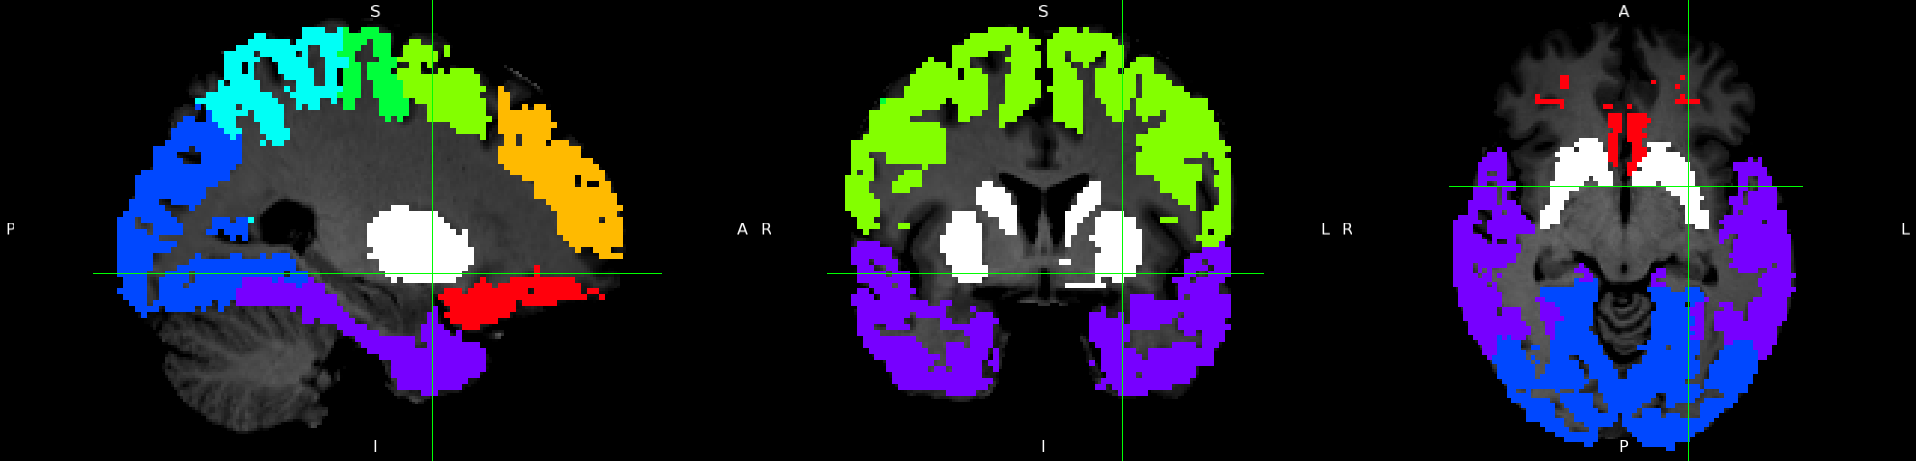
\includegraphics[width=1\textwidth]{rois}
\caption{Basal Ganglia (ROI) \& Cortical Targets}
\label{fig:rois}
\end{figure}

\begin{table}[H]
\centering
\begin{tabular}{|l|l|}
\hline
\textbf{Color} & \textbf{Region} \\ \hline
\begin{tikzpicture}\filldraw[draw=black,fill={rgb,255:red,255;green,255;blue,255}](0,0.15)rectangle(0.25,0.4);\end{tikzpicture} White & Basal Ganglia (ROI) \\ \hline

\begin{tikzpicture}\filldraw[draw=black,fill={rgb,255:red,0;green,255;blue,15}](0,0.15)rectangle(0.25,0.4);\end{tikzpicture} Green & Limbic \\ \hline

\begin{tikzpicture}\filldraw[draw=black,fill={rgb,255:red,255;green,201;blue,126}](0,0.15)rectangle(0.25,0.4);\end{tikzpicture} Brown & Executive \\ \hline

\begin{tikzpicture}\filldraw[draw=black,fill={rgb,255:red,0;green,252;blue,255}](0,0.15)rectangle(0.25,0.4);\end{tikzpicture} Light Blue & Rostral-Motor \\ \hline

\begin{tikzpicture}\filldraw[draw=black,fill={rgb,255:red,251;green,3;blue,255}](0,0.15)rectangle(0.25,0.4);\end{tikzpicture} Purple & Caudal-Motor \\ \hline

\begin{tikzpicture}\filldraw[draw=black,fill={rgb,255:red,253;green,0;blue,0}](0,0.15)rectangle(0.25,0.4);\end{tikzpicture} Red & Parietal \\ \hline

\begin{tikzpicture}\filldraw[draw=black,fill={rgb,255:red,0;green,0;blue,253}](0,0.15)rectangle(0.25,0.4);\end{tikzpicture} Blue & Occipital \\ \hline

\begin{tikzpicture}\filldraw[draw=black,fill={rgb,255:red,255;green,252;blue,0}](0,0.15)rectangle(0.25,0.4);\end{tikzpicture} Yellow & Temporal \\ \hline
\end{tabular}
\caption{Regions Legend}
\label{tab:reglen}
\end{table}

Furthermore, for both the \ac{ROI} and cortical targets, the dataset distinguishes between the right and left hemispheres of the brain. Thus there are actually 2 \ac{ROI}s and $2 \cdot 7=14$ target regions.

\begin{figure}[H]
\centering
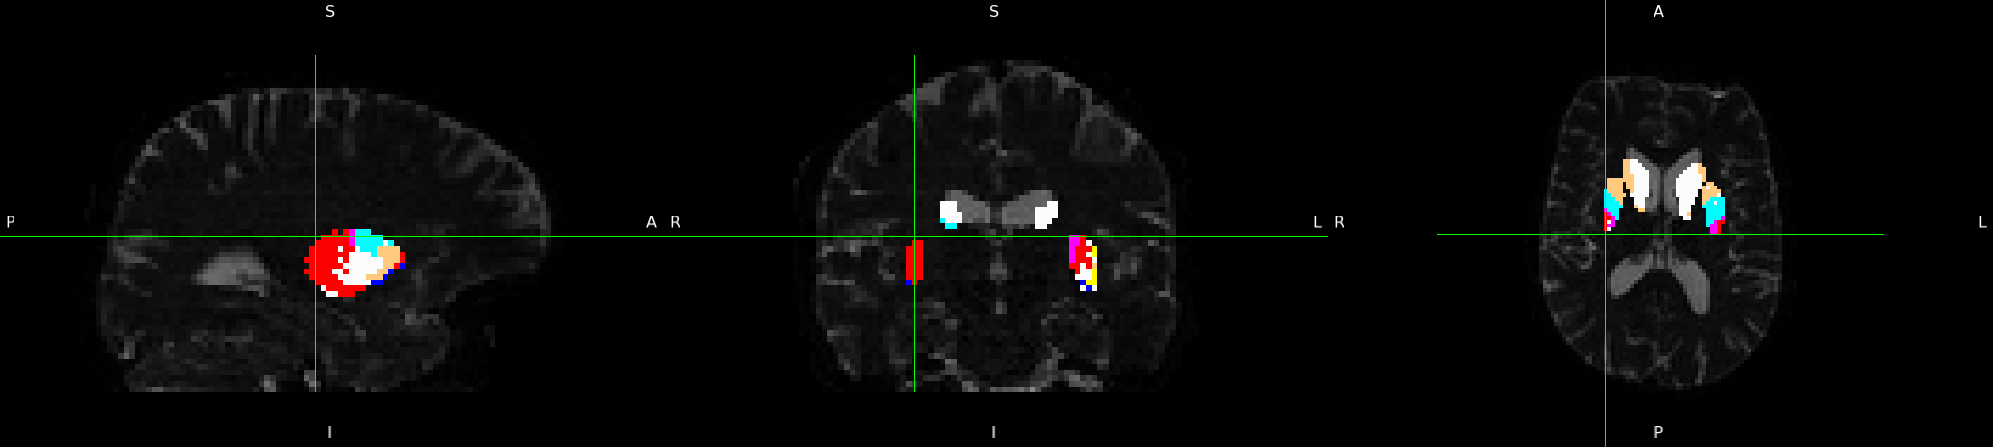
\includegraphics[width=1\textwidth]{conn}
\caption{Connectivity Maps}
\label{fig:conn}
\end{figure}

\section{Objectives}

The end goal is to predict the relative connectivity of the Basal Ganglia to the cortical targets, from the radiomics features of the T1 and T1/T2 images.\par

This being a very complex problem, there is the possibility that the correlation between the connectivity of the brain and the T1, T1/T2 images are too weak to be mapped on this dataset. As from a datascience perspective, 70 records are not much. But from a medical perspective it is substantial as it is very hard to collect uniform, clean data, with permissions to use it for research.\par

A simpler task leading up to the complex end goal, is a model for the simple segmentation of the Basal Ganglia for the subcortical regions Caudate, Putamen and Accumbens. In order to confirm that the radiomics texture of the T1 and T1/T2 images of this dataset are correlated to the segmentation of the Basal Ganglia. This problem is inherently connected to the main goal, as the relative connectivity does obey certain anatomical restrictions, and the subcortical segmentation of the Basal Ganglia is confirmed to be related to the relative connectivity. Thus if this simpler prediction fails, it is almost certain that the complex end goal will fail as well.\par

Another intermediate task, is a model for predicting \ac{FA} and \ac{MD} images. This is also related to the main goal, as these images are computed from the \ac{DTI} images, the same image that the relative connectivity is computed from. But it is inherently simpler, not needing to perform complex algorithms like tractography.\par

The biggest obstacle of this project is the preprocessing of the data, as there are many variations and hyperparameters that can be tuned. An exhaustive search definitely will not be viable, thus the preprocessing and model will needed to be tuned in a waterfall like manner, making educated guesses and comparing model performances across different tries. The main metric to measure model performance, will be the accuracy of the label prediction across voxels, as it should be comparable between all approaches. And pearson correlation will be used as the metric to evaluate the \ac{FA} and \ac{MD} regression predictions.

\section{Motivation}

The motivation for predicting the connectivity maps from the T1 and T1/T2 \ac{MRI} images, is skipping the time and resource consuming process performing \ac{DTI} and tractorgrapy.

\section{State of the Art}





























